\documentclass{beamer}
\usepackage{amsmath}
\usepackage[english]{babel} %set language; note: after changing this, you need to delete all auxiliary files to recompile
\usepackage[utf8]{inputenc} %define file encoding; latin1 is the other often used option
\usepackage{csquotes} % provides context sensitive quotation facilities
\usepackage{graphicx} %allows for inserting figures
\usepackage{booktabs} % for table formatting without vertical lines
\usepackage{textcomp} % allow for example using the Euro sign with \texteuro
\usepackage{stackengine}
\usepackage{wasysym}
\usepackage{tikzsymbols}
\usepackage{textcomp}
\usepackage{xcolor}
\usepackage[dvipsnames]{xcolor}
\usepackage{colortbl}

% ELIMINAR COMANDOS DE NAVEGACION%%%%%%%%%%%
\setbeamertemplate{navigation symbols}

%\newcommand{\bubblethis}[2]{
 %       \tikz[remember picture,baseline]{\node[anchor=base,inner sep=0,outer sep=0]%
 %       (#1) {\underline{#1}};\node[overlay,cloud callout,callout relative pointer={(0.2cm,-0.7cm)},%
 %       aspect=2.5,fill=yellow!90] at ($(#1.north)+(-0.5cm,1.6cm)$) {#2};}%
 %   }%
%\tikzset{face/.style={shape=circle,minimum size=4ex,shading=radial,outer sep=0pt,
 %       inner color=white!50!yellow,outer color= yellow!70!orange}}

%% Some commands to make the code easier
\newcommand{\emoticon}[1][]{%
  \node[face,#1] (emoticon) {};
  %% The eyes are fixed.
  \draw[fill=white] (-1ex,0ex) ..controls (-0.5ex,0.2ex)and(0.5ex,0.2ex)..
        (1ex,0.0ex) ..controls ( 1.5ex,1.5ex)and( 0.2ex,1.7ex)..
        (0ex,0.4ex) ..controls (-0.2ex,1.7ex)and(-1.5ex,1.5ex)..
        (-1ex,0ex)--cycle;}
\newcommand{\pupils}{
  %% standard pupils
  \fill[shift={(0.5ex,0.5ex)},rotate=80] 
       (0,0) ellipse (0.3ex and 0.15ex);
  \fill[shift={(-0.5ex,0.5ex)},rotate=100] 
       (0,0) ellipse (0.3ex and 0.15ex);}

\newcommand{\emoticonname}[1]{
  \node[below=1ex of emoticon,font=\footnotesize,
        minimum width=4cm]{#1};}
\usepackage{scalerel}
\usetikzlibrary{positioning}
\usepackage{xcolor,amssymb}
\newcommand\dangersignb[1][2ex]{%
  \scaleto{\stackengine{0.3pt}{\scalebox{1.1}[.9]{%
  \color{red}$\blacktriangle$}}{\tiny\bfseries !}{O}{c}{F}{F}{L}}{#1}%
}
\newcommand\dangersignw[1][2ex]{%
  \scaleto{\stackengine{0.3pt}{\scalebox{1.1}[.9]{%
  \color{red}$\blacktriangle$}}{\color{white}\tiny\bfseries !}{O}{c}{F}{F}{L}}{#1}%
}
\usepackage{fontawesome} % Social Icons
\usepackage{epstopdf} % allow embedding eps-figures
\usepackage{tikz} % allows drawing figures
\usepackage{amsmath,amssymb,amsthm} %advanced math facilities
\usepackage{lmodern} %uses font that support italic and bold at the same time
\usepackage{hyperref}
\usepackage{tikz}
\hypersetup{
    colorlinks=true,
    linkcolor=blue,
    filecolor=magenta,      
    urlcolor=blue,
}
\usepackage{tcolorbox}
%add citation management using BibLaTeX
\usepackage[citestyle=authoryear-comp, %define style for citations
    bibstyle=authoryear-comp, %define style for bibliography
    maxbibnames=10, %maximum number of authors displayed in bibliography
    minbibnames=1, %minimum number of authors displayed in bibliography
    maxcitenames=3, %maximum number of authors displayed in citations before using et al.
    minnames=1, %maximum number of authors displayed in citations before using et al.
    datezeros=false, % do not print dates with leading zeros
    date=long, %use long formats for dates
    isbn=false,% show no ISBNs in bibliography (applies only if not a mandatory field)
    url=false,% show no urls in bibliography (applies only if not a mandatory field)
    doi=false, % show no dois in bibliography (applies only if not a mandatory field)
    eprint=false, %show no eprint-field in bibliography (applies only if not a mandatory field)
    backend=biber %use biber as the backend; backend=bibtex is less powerful, but easier to install
    ]{biblatex}
\addbibresource{../mybibfile.bib} %define bib-file located one folder higher


\usefonttheme[onlymath]{serif} %set math font to serif ones

\definecolor{beamerblue}{rgb}{0.2,0.2,0.7} %define beamerblue color for later use

%%% defines highlight command to set text blue
\newcommand{\highlight}[1]{{\color{blue}{#1}}}


%%%%%%% commands defining backup slides so that frame numbering is correct

\newcommand{\backupbegin}{
   \newcounter{framenumberappendix}
   \setcounter{framenumberappendix}{\value{framenumber}}
}
\newcommand{\backupend}{
   \addtocounter{framenumberappendix}{-\value{framenumber}}
   \addtocounter{framenumber}{\value{framenumberappendix}}
}

%%%% end of defining backup slides

%Specify figure caption, see also http://tex.stackexchange.com/questions/155738/caption-package-not-working-with-beamer
\setbeamertemplate{caption}{\insertcaption} %redefines caption to remove label "Figure".
%\setbeamerfont{caption}{size=\scriptsize,shape=\itshape,series=\bfseries} %sets figure  caption bold and italic and makes it smaller


\usetheme{Boadilla}

%set options of hyperref package
\hypersetup{
    bookmarksnumbered=true, %put section numbers in bookmarks
    naturalnames=true, %use LATEX-computed names for links
    citebordercolor={1 1 1}, %color of border around cites, here: white, i.e. invisible
    linkbordercolor={1 1 1}, %color of border around links, here: white, i.e. invisible
    colorlinks=true, %color links
    anchorcolor=black, %set color of anchors
    linkcolor=beamerblue, %set link color to beamer blue
    citecolor=blue, %set cite color to beamer blue
    pdfpagemode=UseThumbs, %set default mode of PDF display
    breaklinks=true, %break long links
    pdfstartpage=1 %start at first page
    }


\newtcolorbox{boxA}{
    fontupper = \bf,
    boxrule = 1.5pt,
    colframe = black % frame color
}
\newtcolorbox{boxB}{
    boxrule = 1.5pt,
    colframe = blue!70!black,, % frame color
    colback = blue!7!white,
}

% --------------------
% Overall information
% --------------------
\title[Economía I]{Economía I \vspace{3mm}
\\ Magistral 5 \vspace{3mm} \\ Dentro de la firma II}
\date{}
\author[Victoria Rosino]{Victoria Rosino}
\vspace{0.3cm}
\institute[]{Universidad de San Andrés} 

\begin{document}

\begin{frame}
\vspace{0.3cm}
\titlepage
\centering
\vspace{-0.9cm}

\includegraphics[scale=0.3]{Slides Principios de Economia/Figures/udesa_logo.jpg} 
\end{frame}

\begin{frame}{La última clase terminamos así}
\begin{center}
    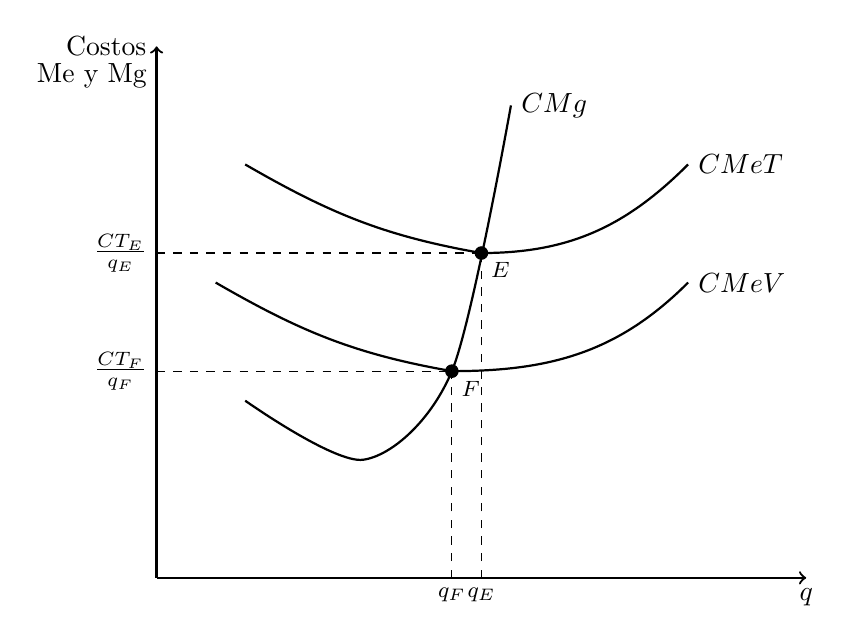
\begin{tikzpicture}[scale=0.75]
        % Ejes
        \draw[thick,->] (0,0) -- (11,0) node[below] {$q$};
        \draw[thick,->] (0,0) -- (0,9) node[left] {Costos};
        \node[left] at (0,8.5) {Me y Mg};
        
        % Curvas
        \draw[thick] (1.5,7) to[out=-30,in=170] (5.5,5.5) to[out=0,in=225] (9,7) node[right] {$CMeT$};;
        \draw[thick] (1,5) to[out=-30,in=170] (5,3.5)to[out=0,in=225] (9,5) node[right] {$CMeV$};;
        \draw[thick] plot[smooth] coordinates {(1.5,3) (3.5,2) (5,3.5) (6,8)} node[right] {$CMg$};

        % Puntos de intersección
        \filldraw (5.5,5.5)  circle (3pt) node[below right] {\footnotesize $E$};
        \filldraw (5,3.5) circle (3pt) node[below right] {\footnotesize $F$};

        % Líneas punteadas horizontales
        \draw[dashed] (0,5.5) -- (5.5,5.5);
        \draw[dashed] (0,3.5) -- (5,3.5);

        % Líneas punteadas verticales
        \draw[dashed] (5.5,0) -- (5.5,5.5) node[above] {};
        \draw[dashed] (5,0) -- (5,3.5) node[above] {};

        % Etiquetas de puntos específicos
        \node[left] at (0,3.5) {\(\frac{CT_F}{q_F}\)};
        \node[left] at (0,5.5) {\(\frac{CT_E}{q_E}\)};
        \node[below] at (5,0) {\footnotesize $q_F$};
        \node[below] at (5.5,0) {\footnotesize $q_E$};

    \end{tikzpicture}
\end{center}
\end{frame}

\begin{frame}
\frametitle{Entonces... ¿cómo decidimos cuánto producir?}
    \begin{itemize}
        \item Por un momento, supongamos que el precio de la pizza es $p$
            \item ¿Me conviene producir una pizza adicional?  
        \begin{itemize}
            \item Si uno aumenta una unidad de producto, recibe $p$
            \item Pero a la vez tiene que pagar el costo de esa unidad ($CMg$)
        \end{itemize}
        \item La diferencia entre el precio $p$ y el $CMg$ es el beneficio marginal
        \item ¿Me conviene producir una pizza adicional?
        \begin{itemize}
            \item Si el beneficio marginal es positivo entonces SÍ conviene producir una pizza adicional
            \item Pero si el beneficio marginal es negativo entonces NO conviene producir una pizza adicional
        \end{itemize} 
        \item ¿Qué significa que el beneficio marginal sea igual 0?
        \begin{boxB}
            \centering
            Para cada cantidad producida, el costo marginal nos dice cuál es el precio mínimo que está dispuesto a aceptar el productor
        \end{boxB}
    \end{itemize}
\end{frame}

\begin{frame}{La curva de oferta de la empresa (corto plazo)}
\begin{center}
    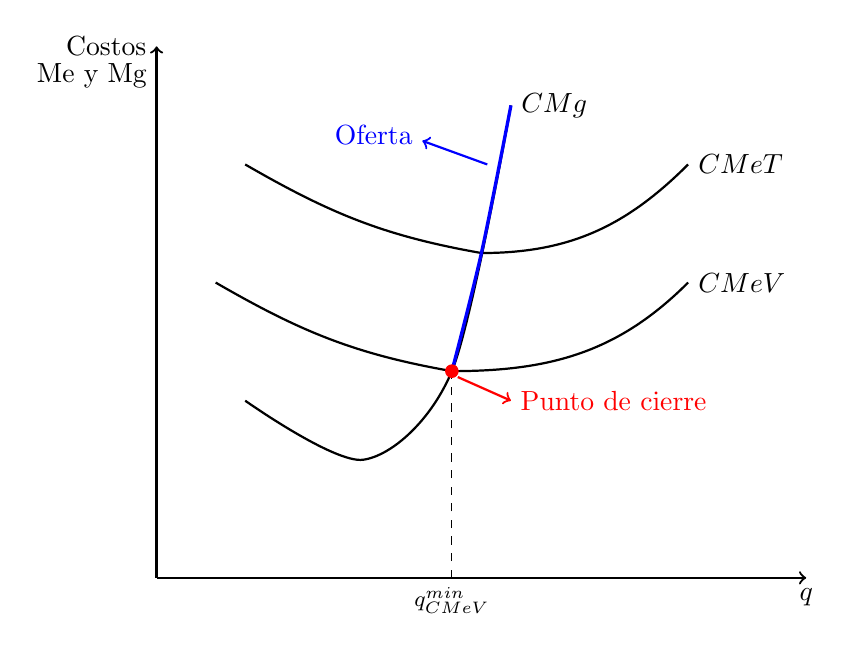
\begin{tikzpicture}[scale=0.75]
        % Ejes
        \draw[thick,->] (0,0) -- (11,0) node[below] {$q$};
        \draw[thick,->] (0,0) -- (0,9) node[left] {Costos};
        \node[left] at (0,8.5) {Me y Mg};
        
        % Curvas
        \draw[thick] (1.5,7) to[out=-30,in=170] (5.5,5.5) to[out=0,in=225] (9,7) node[right] {$CMeT$};;
        \draw[thick] (1,5) to[out=-30,in=170] (5,3.5)to[out=0,in=225] (9,5) node[right] {$CMeV$};;
        \draw[thick] plot[smooth] coordinates {(1.5,3) (3.5,2) (5,3.5) (6,8)} node[right] {$CMg$};

        % Líneas punteadas verticales
        \draw[dashed] (5,0) -- (5,3.5) node[above] {};

        % Etiquetas de puntos específicos
        \node[below] at (5,0) {\footnotesize $q_{CMeV}^{min}$};

        % Oferta
        \draw[very thick, blue] plot[smooth] coordinates {(5,3.5) (5.5,5.5) (6,8)};
        \draw[thick,blue, ->] (5.6,7) -- (4.5,7.4) ;
        \node[left, blue] at (4.5,7.5) {Oferta};

        \filldraw[red] (5,3.5) circle (3pt) node[above] {};  
        \draw[thick,red, ->] (5.1,3.4) -- (6,3);
        \node[right, red] at (6,3) {Punto de cierre};

    \end{tikzpicture}
\end{center}
\end{frame}

\begin{frame}
    \frametitle{Tres facts del analisis marginal}
    \begin{itemize}
        \item La oferta de la firma está dada por la curva de costo marginal, solo en el tramo por encima del punto de cierre (la empresa no produce debajo de este punto)
        \item El punto de cierre es el punto en el cual la empresa está indiferente entre producir y no producir
        \item Si el costo marginal es menor (mayor) que el precio, el nivel de producción debe aumentar (disminuir) hasta el punto en el que el costo marginal sea igual al precio
    \end{itemize}
\end{frame}

\begin{frame}
    \frametitle{Entendiendo el punto de cierre}
    \begin{itemize}
        \item Supongamos que producimos 120 pizzas. El costo total ($CT$) de esas 120 pizzas es \$1.200 (\$400 de costo fijo y \$800 de costo variable). 
        \item ¿Qué pasa si el precio al que vendemos es \$15? \\ \pause
        Los ingresos totales serían: $IT=\$15 \cdot 120 = 1800$
        \\ 
        Y los beneficios: $\Pi= IT -CT=1800-1200=600 $ $\Rightarrow$ ganancia \pause
        \item ¿Y si el precio al que vendemos es \$8? \\ \pause
        $IT = \$8 \cdot 120 = 960$
        \\ 
        $\Pi = 960-1200=-240 $ $\Rightarrow$ pérdida $\Rightarrow$ ¿le conviene producir? \pause \textbf{Sí} \pause
        \item ¿Y si el precio al que vendemos es \$5? \\ \pause
        $IT = \$5 \cdot 120 = 600$
        \\ 
        $\Pi = 600-1200=-600 $ $\Rightarrow$ pérdida $\Rightarrow$ ¿le conviene producir? \pause \textbf{No} \pause
            \begin{boxB}
            \centering
            La empresa produce a partir del precio que le permite cubrir al menos los costos variables
        \end{boxB}
    \end{itemize}
\end{frame}


\begin{frame}
\frametitle{Los costos de largo plazo}
\begin{itemize}
  \item En el largo plazo, la empresa puede ajustar cualquier cantidad de insumos requeridos para la producción. Es decir, \textbf{no hay insumos fijos} y, por ende, tampoco hay costos fijos. 
    \item Los costos de una empresa dependen de su escala y el tipo de tecnología de producción
    \item Empresas grandes pueden ser más rentables que las pequeñas debido diversas ventajas:
    \begin{itemize}
        \item Ventajas tecnológicas: producción a gran escala permite mejorar la especialización y bajar los costos. \vspace{1mm}
        \item Ventajas de costos: por ejemplo, empresas grandes, con mayor poder de negociación, pueden comprar recursos en términos más favorables.  \vspace{1mm}
        \item Ventajas de demanda: por ejemplo, efectos de red (valor de la producción aumenta con el número de usuarios).  \vspace{1mm}
    \end{itemize}
\end{itemize}
\end{frame}

\begin{frame}
\frametitle{Rendimientos a escala}
\begin{itemize}
    \item ¿Qué sucede con la producción cuando aumentamos la cantidad de insumos productivos en la misma proporción?
    \begin{itemize}
        \item La producción aumenta pero... ¿cuánto aumenta?
    \end{itemize}
    \item Si la producción aumenta más que proporcionalmente, entonces la función de producción exhibe rendimientos crecientes a escala (Economías de escala o costos decrecientes a escala)
    \item Si la producción aumenta proporcionalmente, entonces la función de producción exhibe rendimientos constantes a escala (Costos constantes a escala)
    \item Si la producción aumenta menos que proporcionalmente, entonces la función de producción exhibe rendimientos decrecientes a escala (Deseconomías de escala o costos crecientes a escala)
\end{itemize}
\end{frame}

\begin{frame}
    \frametitle{Rendimientos a escala}
    Esto se resume en el siguiente cociente:
    \[ \frac{\Delta \% Q}{\Delta \% I} \]
    \begin{itemize}
        \item Si el cociente es mayor a 1, entonces hay rendimientos crecientes a escala
        \item Si el cociente es igual a 1, entonces hay rendimientos constantes a escala
        \item Si el cociente es menor a 1, entonces hay rendimientos decrecientes a escala
    \end{itemize}

\end{frame}

\begin{frame}{La pizzería en el largo plazo}
    
\begin{center}
    \begin{tikzpicture}
        % Ejes
        \draw[thick,->] (0,0) -- (8,0) node[below] {\textbf{Pizzas}};
        \draw[thick,->] (0,0) -- (0,6) node[left] {\textbf{Costos}};

        % Curva 1
        \draw[blue, thick] (0.2,4) to[out=-60,in=180] (1.75,2.7) to[out=0,in=240] (3.5,4);
        \node at (1.8,3.9) {Haciendo pizzas};
        \node at (1.8,3.5) {en casa};

        % Curva 2
        \only<3->{
        \draw[blue, thick] (2.5,3) to[out=-60,in=180] (4.25,1.7) to[out=0,in=240] (6,3);
        \node at (4.2,3) {Pizzas en};
        \node at (4.2,2.6) {varios locales};
        }

        % Curva 3
        \only<4->{
        \draw[blue, thick] (5,4) to[out=-60,in=180] (6.75,2.7) to[out=0,in=240] (8.5,4);
        \node at (6.75,3.9) {El imperio};
        \node at (6.75,3.5) {de la pizzas};
        }
    \end{tikzpicture}
\end{center}
\end{frame}

\begin{frame}
\frametitle{Costos en el largo plazo}
\begin{center}
    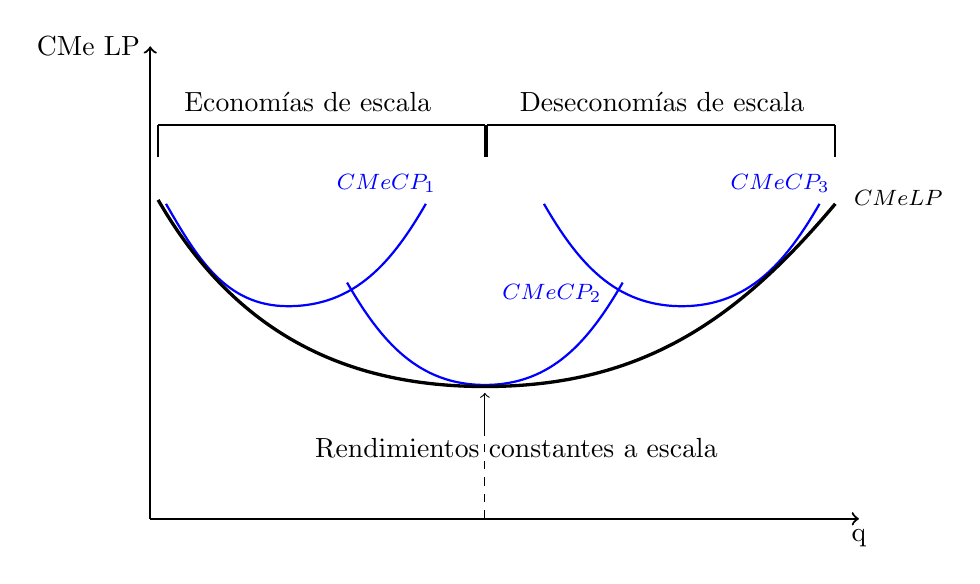
\begin{tikzpicture}
        % Ejes
        \draw[thick,->] (0,0) -- (9,0) node[below] {q};
        \draw[thick,->] (0,0) -- (0,6) node[left] {CMe LP};

        % Curva 1
        \draw[blue, thick] (0.2,4) to[out=-60,in=180] (1.75,2.7) to[out=0,in=240] (3.5,4);
        \node[below] at (3,4.5) {\footnotesize \textcolor{blue}{$CMeCP_1$}};
        
        % Curva 2
        \draw[blue, thick] (2.5,3) to[out=-60,in=180] (4.25,1.7) to[out=0,in=240] (6,3);
        \node[below] at (5.1,3.1) {\footnotesize \textcolor{blue}{$CMeCP_2$}};
        
        % Curva 3
        \draw[blue, thick] (5,4) to[out=-60,in=180] (6.75,2.7) to[out=0,in=240] (8.5,4);
        \node[below] at (8,4.5) {\footnotesize \textcolor{blue}{$CMeCP_3$}};

        % Curva de LP
        \draw[very thick] (0.1,4.05) to[out=-60,in=180] (4.25,1.68) to[out=0,in=230] (8.7,4);
        \node[below] at (9.5,4.3) {\footnotesize $CMeLP$};

        \draw[thick] (0.1,5) -- (4.25,5);
        \draw[thick] (4.25,4.6) -- (4.25,5);
        \draw[thick] (0.1,4.6) -- (0.1,5);
        \node at (2,5.3) {Economías de escala}; 

        \draw[thick] (4.28,5) -- (8.7,5);
        \draw[thick] (4.28,4.6) -- (4.28,5);
        \draw[thick] (8.7,4.6) -- (8.7,5);
        \node at (6.5,5.3) {Deseconomías de escala}; 

        \draw[dashed] (4.25,0) -- (4.25,1.68);
        \draw[->] (4.25,1.1) -- (4.25,1.6);
        \node at (4.65,0.9) {Rendimientos constantes a escala};
    \end{tikzpicture}
\end{center}
\end{frame}


\begin{frame}
    \frametitle{La oferta del mercado}
    \begin{itemize}
        \item  Hasta ahora estudiamos cómo las condiciones tecnológicas y los costos de producción determinan las decisiones de la empresa. 
        \item Conociendo las ofertas individuales de las firmas, deberíamos tener en cuenta cuántas empresas producen el bien en cuestión para obtener su oferta del mercado. 
    \end{itemize}
    
\renewcommand{\arraystretch}{1.2} % Espaciado entre filas
\begin{table}[h]
    \centering
    \rowcolors{2}{gray!10}{white} % Alternar colores en las filas
    \setlength{\arrayrulewidth}{1pt} % Grosor de líneas
    \arrayrulecolor{black} % Color de líneas
    \begin{tabular}{|c|c|c|c|c|}
        \hline
        \rowcolor{blue!20} % Color de la primera fila (encabezado)
        \textbf{P} & \textbf{QEmpresa$_1$} & \textbf{QEmpresa$_2$} & \textbf{QEmpresa$_3$} & \textbf{QTotal} \\
        \hline
        0  & 4  & 0  & 0  & 4  \\
        10 & 6  & 0  & 10 & 16 \\
        20 & 8  & 0  & 20 & 28 \\
        30 & 10 & 0  & 30 & 40 \\
        40 & 12 & 20 & 40 & 72 \\
        50 & 14 & 30 & 50 & 94 \\
        60 & 16 & 40 & 60 & 116 \\
        \hline
    \end{tabular}
\end{table}
\end{frame}

\begin{frame}
    \frametitle{La oferta del mercado}
\begin{center}
    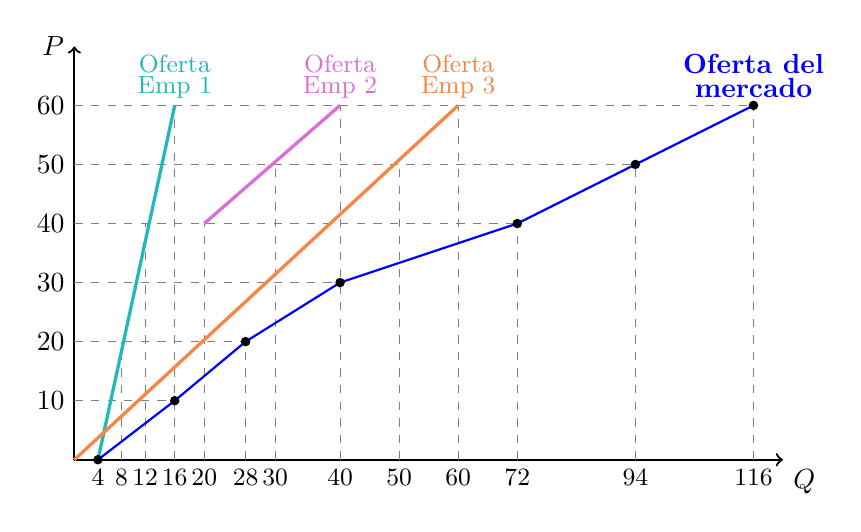
\begin{tikzpicture}[scale=0.75]
        % Ejes
        \draw[thick,->] (0,0) -- (12,0) node[below right] { ${Q}$};
        \draw[thick,->] (0,0) -- (0,7) node[left] { ${P}$};

        % Lineas punteadas
        \draw[dashed, gray] (0,6) -- (11.5,6);
        \draw[dashed, gray] (0,5) -- (9.5,5);
        \draw[dashed, gray] (0,4) -- (7.5,4);
        \draw[dashed, gray] (0,3) -- (4.5,3);
        \draw[dashed, gray] (0,2) -- (2.9,2);
        \draw[dashed, gray] (0,1) -- (1.7,1);

        \draw[dashed, gray] (11.5,0) -- (11.5,6);
        \draw[dashed, gray] (9.5,0) -- (9.5,5);
        \draw[dashed, gray] (7.5,0) -- (7.5,4);
        \draw[dashed, gray] (6.5,0) -- (6.5,6);
        \draw[dashed, gray] (5.5,0) -- (5.5,5);
        \draw[dashed, gray] (4.5,0) -- (4.5,6);
        \draw[dashed, gray] (3.4,0) -- (3.4,5);
        \draw[dashed, gray] (2.2,0) -- (2.2,4);
        \draw[dashed, gray] (2.9,0) -- (2.9,2);
        \draw[dashed, gray] (1.7,0) -- (1.7,6);
        \draw[dashed, gray] (1.2,0) -- (1.2,4);
        \draw[dashed, gray] (0.8,0) -- (0.8,2);


        % Curvas de oferta de los empresarios
        \draw[very thick, BlueGreen] (0.4,0) -- (1.7,6);
        \node at (1.7,6.7) {\small \textcolor{BlueGreen}{Oferta}};
        \node at (1.7,6.3) {\small \textcolor{BlueGreen}{Emp 1}}; 
        \draw[very thick, Orchid] (2.2,4) -- (4.5,6);         
        \node at (4.5,6.7) {\small \textcolor{Orchid}{Oferta}};
        \node at (4.5,6.3) {\small \textcolor{Orchid}{Emp 2}}; 
        \draw[very thick, Peach] (0,0) -- (6.5,6);
        \node at (6.5,6.7) {\small \textcolor{Peach}{Oferta}};
        \node at (6.5,6.3) {\small \textcolor{Peach}{Emp 3}}; 

        % Oferta del mercado (azul)
        \draw[thick,Blue] (0.4,0) -- (1.7,1) -- (2.9,2) -- (4.5,3) -- (7.5,4) -- (9.5,5) -- (11.5,6);
        \node at (11.5, 6.7) {\textcolor{Blue}{\textbf{Oferta del}}};
        \node at (11.5, 6.3)  {\textcolor{Blue}{\textbf{mercado}}};

        % Puntos en la oferta del mercado
        \foreach \x/\y in {0.4/0, 1.7/1, 2.9/2, 4.5/3, 7.5/4, 9.5/5, 11.5/6} {
            \filldraw[black] (\x,\y) circle (2pt);
        }

        % Etiquetas en el eje X (cantidades)
        \node[below] at (0.4,0) {\small 4};
        \node[below] at (0.8,0) {\small8};
        \node[below] at (1.2,0) {\small12};
        \node[below] at (1.7,0) {\small16};
        \node[below] at (2.2,0) {\small20};
        \node[below] at (2.9,0) {\small28};
        \node[below] at (3.4,0) {\small30};
        \node[below] at (4.5,0) {\small40};
        \node[below] at (5.5,0) {\small50};
        \node[below] at (6.5,0) {\small60};
        \node[below] at (7.5,0) {\small72};
        \node[below] at (9.5,0) {\small94};
        \node[below] at (11.5,0) {\small116};

        % Etiquetas en el eje Y (precios)
        \node[left] at (0,1) {10};
        \node[left] at (0,2) {20};
        \node[left] at (0,3) {30};
        \node[left] at (0,4) {40};
        \node[left] at (0,5) {50};
        \node[left] at (0,6) {60};

    \end{tikzpicture}
\end{center}
\centering
La oferta de mercado se obtiene sumando las cantidades que están dispuestas a producir cada una de las empresas a cada precio.
\end{frame}

\begin{frame}
    \frametitle{Qu{e es la oferta?}}
\begin{itemize}
    \item  La oferta del mercado refleja la cantidad de bienes que se va ofrecer de manera conjunta en el mercado a cada precio.
    \item Alternativamente, se puede interpretar como la mínima disposición a cobrar que tienen los productores para cada cantidad del producto que venden.
\end{itemize}

    \begin{center}
        \begin{tikzpicture}[scale=0.65]
        \draw[thick,->] (0,0) -- (8,0) node[below] {$Q$};
        \draw[thick,->] (0,0) -- (0,6.5) node[left] {$P$};
        \draw [thick] (1,2) -- (7,5);
        \node [right] at (7.1,5.2) {Oferta};
        % Punto A
        \node [right] at (3,3.6) {$A$};
        \fill (3.2,3.1) circle (3pt);
        \draw[dashed, gray] (3.2,0) -- (3.2,3.1);
        \draw[dashed, gray] (0,3.1) -- (3.2,3.1);
        \node[below] at (3.2,0) {40};
        \node[left] at (0,3.1) {30};
        \end{tikzpicture}
    \end{center}
\end{frame}

\begin{frame}
\frametitle{Desplazamientos \textbf{sobre} la curva de oferta}

    \begin{itemize}
        \item Si cambia el \textbf{precio} del producto, se modifica su \textbf{cantidad ofrecida}.
        \item La curva de oferta no se modifica, nos desplazamos \textbf{sobre} la curva.\vspace{1mm}
    \end{itemize}
    \begin{center}
        \begin{tikzpicture}[scale=0.8]
        \draw[thick,->] (0,0) -- (8,0) node[below] {$Q$};
        \draw[thick,->] (0,0) -- (0,6.5) node[left] {$P$};
        \draw [thick] (1,2) -- (7,5);
        \node [right] at (7.1,5.2) {Oferta};

        % Punto A
        \node [right] at (3.1,3.5) {$A$};
        \fill (3.2,3.1) circle (3pt);
        \draw[dashed, gray] (3.2,0) -- (3.2,3.1);
        \draw[dashed, gray] (0,3.1) -- (3.2,3.1);
        \node[below] at (3.2,0) {40};
        \node[left] at (0,3.1) {30};
        
        % Punto B
        \node [right] at (5.5,4.7) {$B$};
        \fill (5.6,4.3) circle (3pt);
        \draw[dashed, gray] (5.6,0) -- (5.6,4.3);
        \draw[dashed, gray] (0,4.3) -- (5.6,4.3);
        \node[below] at (5.6,0) {60};
        \node[left] at (0,4.3) {40};
        \end{tikzpicture}
    \end{center}

\end{frame}

\begin{frame}{Factores que afectan a la curva de oferta}
    \begin{itemize}
        \item La tecnología y sus cambios
        \item El precio de los insumos requeridos para la producción
        \item Los precios de bienes relacionados
        \item El número de vendedores que hay en el mercado
        \item Las distintas políticas gubernamentales (por ejemplo, los impuestos)
        \item Las expectativas de los productores
        \item Otras influencias externas (por ejemplo, el clima en el caso de productos agrícolas)  

    \begin{boxB}
    \begin{center}
      No confundir cambios en la oferta con cambios \\ en las cantidades ofrecidas
    \end{center}
    \end{boxB}
    \end{itemize}
\end{frame}

\begin{frame}
\frametitle{Algunos ejemplos}
    \begin{center}
    
\includegraphics[scale=0.35]{Slides Principios de Economia/Figures/Magistral_06/M6.1.png}
    \end{center}
\end{frame}

\begin{frame}
\frametitle{Algunos ejemplos}
    \begin{center}
    
\includegraphics[scale=0.35]{Slides Principios de Economia/Figures/Magistral_06/M6.2.png}
    \end{center}
\end{frame}

\begin{frame}
\frametitle{Algunos ejemplos}
    \begin{center}
    
\includegraphics[scale=0.5]{Slides Principios de Economia/Figures/Magistral_06/M6.3.png}
    \end{center}
\end{frame}

\begin{frame}
\frametitle{Algunos ejemplos}
    \begin{center}
    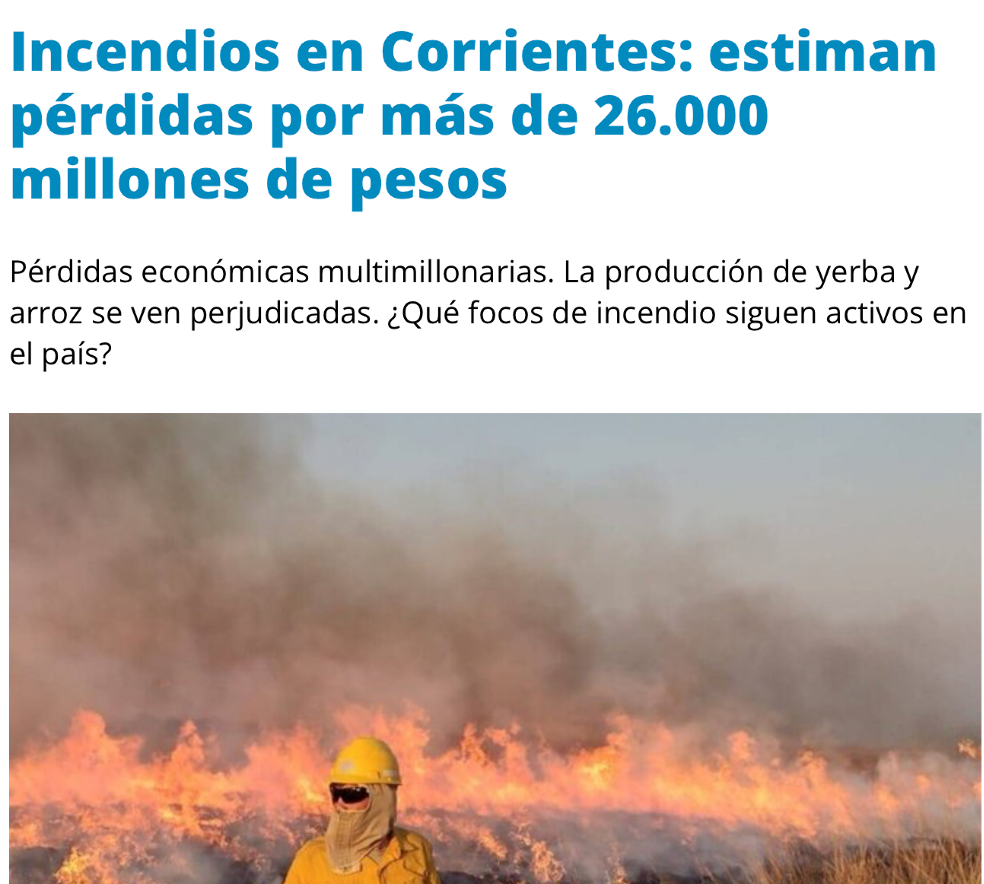
\includegraphics[scale=0.45]{Slides Principios de Economia/Figures/Magistral_06/M6.4.png}
    \end{center}
\end{frame}
\end{document}





